\documentclass{ximera}  


%\usepackage{todonotes}
%\usepackage{mathtools} %% Required for wide table Curl and Greens
%\usepackage{cuted} %% Required for wide table Curl and Greens
\newcommand{\todo}{}

\usepackage{esint} % for \oiint
\ifxake%%https://math.meta.stackexchange.com/questions/9973/how-do-you-render-a-closed-surface-double-integral
\renewcommand{\oiint}{{\large\bigcirc}\kern-1.56em\iint}
\fi


\graphicspath{
  {./}
  {jpg}
  {ximeraTutorial/}
  {basicPhilosophy/}
  {functionsOfSeveralVariables/}
  {normalVectors/}
  {lagrangeMultipliers/}
  {vectorFields/}
  {greensTheorem/}
  {shapeOfThingsToCome/}
  {dotProducts/}
  {partialDerivativesAndTheGradientVector/}
  {../productAndQuotientRules/exercises/}
  {../motionAndPathsInSpace/exercises/}
  {../normalVectors/exercisesParametricPlots/}
  {../continuityOfFunctionsOfSeveralVariables/exercises/}
  {../partialDerivativesAndTheGradientVector/exercises/}
  {../directionalDerivativeAndChainRule/exercises/}
  {../commonCoordinates/exercisesCylindricalCoordinates/}
  {../commonCoordinates/exercisesSphericalCoordinates/}
  {../greensTheorem/exercisesCurlAndLineIntegrals/}
  {../greensTheorem/exercisesDivergenceAndLineIntegrals/}
  {../shapeOfThingsToCome/exercisesDivergenceTheorem/}
  {../greensTheorem/}
  {../shapeOfThingsToCome/}
  {../separableDifferentialEquations/exercises/}
  {vectorFields/}
}

\newcommand{\mooculus}{\textsf{\textbf{MOOC}\textnormal{\textsf{ULUS}}}}

\usepackage{tkz-euclide}\usepackage{tikz}
\usepackage{tikz-cd}
\usetikzlibrary{arrows}
\tikzset{>=stealth,commutative diagrams/.cd,
  arrow style=tikz,diagrams={>=stealth}} %% cool arrow head
\tikzset{shorten <>/.style={ shorten >=#1, shorten <=#1 } } %% allows shorter vectors

\usetikzlibrary{backgrounds} %% for boxes around graphs
\usetikzlibrary{shapes,positioning}  %% Clouds and stars
\usetikzlibrary{matrix} %% for matrix
\usepgfplotslibrary{polar} %% for polar plots
\usepgfplotslibrary{fillbetween} %% to shade area between curves in TikZ
\usetkzobj{all}
\usepackage[makeroom]{cancel} %% for strike outs
%\usepackage{mathtools} %% for pretty underbrace % Breaks Ximera
%\usepackage{multicol}
\usepackage{pgffor} %% required for integral for loops



%% http://tex.stackexchange.com/questions/66490/drawing-a-tikz-arc-specifying-the-center
%% Draws beach ball
\tikzset{pics/carc/.style args={#1:#2:#3}{code={\draw[pic actions] (#1:#3) arc(#1:#2:#3);}}}



\usepackage{array}
\setlength{\extrarowheight}{+.1cm}
\newdimen\digitwidth
\settowidth\digitwidth{9}
\def\divrule#1#2{
\noalign{\moveright#1\digitwidth
\vbox{\hrule width#2\digitwidth}}}





\newcommand{\RR}{\mathbb R}
\newcommand{\R}{\mathbb R}
\newcommand{\N}{\mathbb N}
\newcommand{\Z}{\mathbb Z}

\newcommand{\sagemath}{\textsf{SageMath}}


%\renewcommand{\d}{\,d\!}
\renewcommand{\d}{\mathop{}\!d}
\newcommand{\dd}[2][]{\frac{\d #1}{\d #2}}
\newcommand{\pp}[2][]{\frac{\partial #1}{\partial #2}}
\renewcommand{\l}{\ell}
\newcommand{\ddx}{\frac{d}{\d x}}

\newcommand{\zeroOverZero}{\ensuremath{\boldsymbol{\tfrac{0}{0}}}}
\newcommand{\inftyOverInfty}{\ensuremath{\boldsymbol{\tfrac{\infty}{\infty}}}}
\newcommand{\zeroOverInfty}{\ensuremath{\boldsymbol{\tfrac{0}{\infty}}}}
\newcommand{\zeroTimesInfty}{\ensuremath{\small\boldsymbol{0\cdot \infty}}}
\newcommand{\inftyMinusInfty}{\ensuremath{\small\boldsymbol{\infty - \infty}}}
\newcommand{\oneToInfty}{\ensuremath{\boldsymbol{1^\infty}}}
\newcommand{\zeroToZero}{\ensuremath{\boldsymbol{0^0}}}
\newcommand{\inftyToZero}{\ensuremath{\boldsymbol{\infty^0}}}



\newcommand{\numOverZero}{\ensuremath{\boldsymbol{\tfrac{\#}{0}}}}
\newcommand{\dfn}{\textbf}
%\newcommand{\unit}{\,\mathrm}
\newcommand{\unit}{\mathop{}\!\mathrm}
\newcommand{\eval}[1]{\bigg[ #1 \bigg]}
\newcommand{\seq}[1]{\left( #1 \right)}
\renewcommand{\epsilon}{\varepsilon}
\renewcommand{\phi}{\varphi}


\renewcommand{\iff}{\Leftrightarrow}

\DeclareMathOperator{\arccot}{arccot}
\DeclareMathOperator{\arcsec}{arcsec}
\DeclareMathOperator{\arccsc}{arccsc}
\DeclareMathOperator{\si}{Si}
\DeclareMathOperator{\scal}{scal}
\DeclareMathOperator{\sign}{sign}


%% \newcommand{\tightoverset}[2]{% for arrow vec
%%   \mathop{#2}\limits^{\vbox to -.5ex{\kern-0.75ex\hbox{$#1$}\vss}}}
\newcommand{\arrowvec}[1]{{\overset{\rightharpoonup}{#1}}}
%\renewcommand{\vec}[1]{\arrowvec{\mathbf{#1}}}
\renewcommand{\vec}[1]{{\overset{\boldsymbol{\rightharpoonup}}{\mathbf{#1}}}\hspace{0in}}

\newcommand{\point}[1]{\left(#1\right)} %this allows \vector{ to be changed to \vector{ with a quick find and replace
\newcommand{\pt}[1]{\mathbf{#1}} %this allows \vec{ to be changed to \vec{ with a quick find and replace
\newcommand{\Lim}[2]{\lim_{\point{#1} \to \point{#2}}} %Bart, I changed this to point since I want to use it.  It runs through both of the exercise and exerciseE files in limits section, which is why it was in each document to start with.

\DeclareMathOperator{\proj}{\mathbf{proj}}
\newcommand{\veci}{{\boldsymbol{\hat{\imath}}}}
\newcommand{\vecj}{{\boldsymbol{\hat{\jmath}}}}
\newcommand{\veck}{{\boldsymbol{\hat{k}}}}
\newcommand{\vecl}{\vec{\boldsymbol{\l}}}
\newcommand{\uvec}[1]{\mathbf{\hat{#1}}}
\newcommand{\utan}{\mathbf{\hat{t}}}
\newcommand{\unormal}{\mathbf{\hat{n}}}
\newcommand{\ubinormal}{\mathbf{\hat{b}}}

\newcommand{\dotp}{\bullet}
\newcommand{\cross}{\boldsymbol\times}
\newcommand{\grad}{\boldsymbol\nabla}
\newcommand{\divergence}{\grad\dotp}
\newcommand{\curl}{\grad\cross}
%\DeclareMathOperator{\divergence}{divergence}
%\DeclareMathOperator{\curl}[1]{\grad\cross #1}
\newcommand{\lto}{\mathop{\longrightarrow\,}\limits}

\renewcommand{\bar}{\overline}

\colorlet{textColor}{black}
\colorlet{background}{white}
\colorlet{penColor}{blue!50!black} % Color of a curve in a plot
\colorlet{penColor2}{red!50!black}% Color of a curve in a plot
\colorlet{penColor3}{red!50!blue} % Color of a curve in a plot
\colorlet{penColor4}{green!50!black} % Color of a curve in a plot
\colorlet{penColor5}{orange!80!black} % Color of a curve in a plot
\colorlet{penColor6}{yellow!70!black} % Color of a curve in a plot
\colorlet{fill1}{penColor!20} % Color of fill in a plot
\colorlet{fill2}{penColor2!20} % Color of fill in a plot
\colorlet{fillp}{fill1} % Color of positive area
\colorlet{filln}{penColor2!20} % Color of negative area
\colorlet{fill3}{penColor3!20} % Fill
\colorlet{fill4}{penColor4!20} % Fill
\colorlet{fill5}{penColor5!20} % Fill
\colorlet{gridColor}{gray!50} % Color of grid in a plot

\newcommand{\surfaceColor}{violet}
\newcommand{\surfaceColorTwo}{redyellow}
\newcommand{\sliceColor}{greenyellow}




\pgfmathdeclarefunction{gauss}{2}{% gives gaussian
  \pgfmathparse{1/(#2*sqrt(2*pi))*exp(-((x-#1)^2)/(2*#2^2))}%
}


%%%%%%%%%%%%%
%% Vectors
%%%%%%%%%%%%%

%% Simple horiz vectors
\renewcommand{\vector}[1]{\left\langle #1\right\rangle}


%% %% Complex Horiz Vectors with angle brackets
%% \makeatletter
%% \renewcommand{\vector}[2][ , ]{\left\langle%
%%   \def\nextitem{\def\nextitem{#1}}%
%%   \@for \el:=#2\do{\nextitem\el}\right\rangle%
%% }
%% \makeatother

%% %% Vertical Vectors
%% \def\vector#1{\begin{bmatrix}\vecListA#1,,\end{bmatrix}}
%% \def\vecListA#1,{\if,#1,\else #1\cr \expandafter \vecListA \fi}

%%%%%%%%%%%%%
%% End of vectors
%%%%%%%%%%%%%

%\newcommand{\fullwidth}{}
%\newcommand{\normalwidth}{}



%% makes a snazzy t-chart for evaluating functions
%\newenvironment{tchart}{\rowcolors{2}{}{background!90!textColor}\array}{\endarray}

%%This is to help with formatting on future title pages.
\newenvironment{sectionOutcomes}{}{}



%% Flowchart stuff
%\tikzstyle{startstop} = [rectangle, rounded corners, minimum width=3cm, minimum height=1cm,text centered, draw=black]
%\tikzstyle{question} = [rectangle, minimum width=3cm, minimum height=1cm, text centered, draw=black]
%\tikzstyle{decision} = [trapezium, trapezium left angle=70, trapezium right angle=110, minimum width=3cm, minimum height=1cm, text centered, draw=black]
%\tikzstyle{question} = [rectangle, rounded corners, minimum width=3cm, minimum height=1cm,text centered, draw=black]
%\tikzstyle{process} = [rectangle, minimum width=3cm, minimum height=1cm, text centered, draw=black]
%\tikzstyle{decision} = [trapezium, trapezium left angle=70, trapezium right angle=110, minimum width=3cm, minimum height=1cm, text centered, draw=black]




 
\title{Transmission line impedance and reflection coefficient} 
\author{Milica Markovic} 
\outcome{Derive and calculate the transmission line impedance and reflection coefficient. Relate reflection coefficient to impedance.}
\begin{document}  
\begin{abstract}  

\end{abstract}  
\maketitle    











\section{Relating forward and backward current and voltage waves on
the transmission line}


In equations \ref{eq4}-\ref{eq5} $\tilde{V}_0^+$ and $\tilde{V}_0^-$ are the phasors of forward and
reflected going voltage waves, and $\tilde{I}_0^+$ and $\tilde{I}_0^-$ are the phasors of forward and
reflected current waves. This section will relate the phasors of voltage and
current waves with transmission-line impedance.


\begin{eqnarray}
\tilde{V}(z)=\tilde{V}_0^+ e^{-\gamma z} + \tilde{V}_0^- e^{\gamma z}\label{eq4} \\
I(z)=\tilde{I}_0^+ e^{-\gamma z} + \tilde{I}_0^- e^{\gamma z}\label{eq5}
\end{eqnarray}




When substitute the voltage wave equation into Telegrapher's  Equations
\ref{te11}. The equation is repeated here  Eq.\ref{te12new}-\ref{te12new1}.




\begin{eqnarray}
-\frac{\partial \tilde{V}(z)}{\partial z} = (R+j\omega L) I(z) \label{te12new} \\
\gamma \tilde{V}_0^+ e^{-\gamma z} - \gamma \tilde{V}_0^- e^{\gamma z} = (R+ j \omega
L) I(z) \label{te12new1}
\end{eqnarray}

We now rearrange Eq.\ref{te12new1}

\begin{eqnarray}
I(z)=\frac{\gamma}{R+j\omega L} ( \tilde{V}_0^+ e^{-\gamma z} + \tilde{V}_0^-
 e^{\gamma z})  \nonumber  \\
I(z)=\frac{\gamma \tilde{V}_0^+}{R+ j \omega L} e^{-\gamma z} - \frac{\gamma \tilde{V}_0^-}{R+ j \omega L} e^{\gamma z} \label{eq3}
\end{eqnarray}

Now we compare Eq.\ref{eq3} with the Eq.\ref{eq5}. For two transcendental equations to be equal, the coefficients next to exponential terms have to be the same.

\begin{eqnarray}
\tilde{I}_0^+=\frac{\gamma \tilde{V}_0^+}{R+ j \omega L} \nonumber  \\
\tilde{I}_0^-= - \frac{\gamma \tilde{V}_0^-}{R+ j \omega L} \nonumber
\end{eqnarray}

We can define the characteristic impedance of a transmission line as
the ratio of the voltage to the current amplitude of the forward-going
wave.


\begin{eqnarray}
Z_0=\frac{\tilde{V}_0^+}{ \tilde{I}_0^+} \nonumber   \\ \nonumber
Z_0=\frac{R+j\omega L}{\gamma} \nonumber   \\ \nonumber
Z_0=\sqrt{\frac{R+j\omega L}{G+ j\omega C}}
\end{eqnarray}






\section{Voltage Reflection Coefficient, Lossless Case}

The equations for the voltage and current on the transmission line we
derived so far are

\begin{eqnarray}
\tilde{V}(z)=\tilde{V}_0^+ e^{-j \beta z} +\tilde{V}_0^- e^{j \beta z} \label{vtl} \\ \label{ctl}
I(z)=\frac{\tilde{V}_0^+}{Z_0} e^{- j \beta z} - \frac{\tilde{V}_0^-}{Z_0} e^{j \beta z}
\end{eqnarray}



\begin{figure}[htbp]
\begin{center}
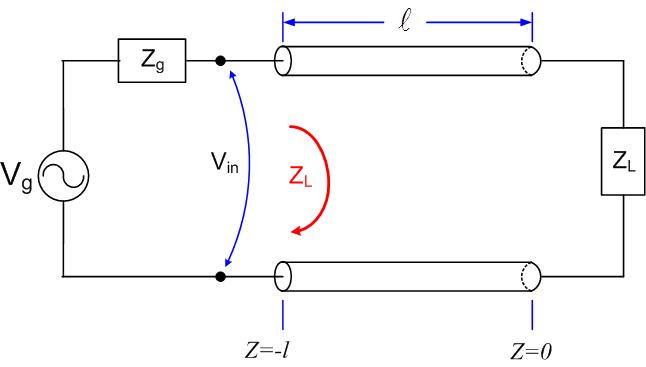
\includegraphics[scale=0.3]{../jpg/trline.jpg}
%\strut\psfig{figure=trline.ps,width=3cm} \\
\end{center}
\caption{Transmission Line connects generator and the load.}
\label{wind1}
\end{figure}





At $z=0$ the impedance of the load has to be

\begin{eqnarray}
Z_L=\frac{V(0)}{I(0)} \nonumber 
\end{eqnarray}

Substitute the boundary condition in Eq.\ref{vtl}

\begin{eqnarray}
Z_L=Z_0 \frac{\tilde{V}_0^+ + \tilde{V}_0^-}{\tilde{V}_0^+ - \tilde{V}_0^-}
\end{eqnarray}


We can now solve the above equation for $\tilde{V}_0^-$

\begin{eqnarray}
\frac{Z_L}{Z_0} (\tilde{V}_0^+ - \tilde{V}_0^-) = \tilde{V}_0^+ + \tilde{V}_0^- \nonumber \\
(\frac{Z_L}{Z_0}-1)\tilde{V}_0^+ =(\frac{Z_L}{Z_0}+1) \tilde{V}_0^- \nonumber \\
\frac{\tilde{V}_0^-}{\tilde{V}_0^+} = \frac{\frac{Z_L}{Z_0}-1  }{ \frac{Z_L}{Z_0}+1 } = \frac{z_L-1}{z_L+1}
\nonumber \\
\Gamma=\frac{\tilde{V}_0^-}{\tilde{V}_0^+} = \frac{Z_L -Z_0}{Z_L +Z_0}
\end{eqnarray}

The quantity $\frac{\tilde{V}_0^-}{\tilde{V}_0^+}$ is called voltage reflection
coefficient $\Gamma$. $\Gamma$ relates the reflected and incident voltage
phasor. The voltage reflection coefficient is, in general, a complex number,
it has a magnitude and a phase.

 Lowercase $z_L$ is called the 
"normalized load impedance". It is the actual impedance divided by the transmission line impedance $z_L=\frac{Z_L}{Z_0}$. For example, if the load impedance is $Z_L=100 \Omega$, and the transmission-line impedance is $Z)=50 \Omega$, then the normalized impedance is $z_L=\frac{100 \Omega}{50 \Omega}=2$. Normalized impedance is a unitless quantity.



\subsubsection{Example}


 \begin{enumerate}
\item 100\,$\Omega$ transmission line is terminated in a series
connection of a 50\,$\Omega$ resistor and 10\,pF capacitor. The frequency
of operation is 100\,MHz. Find the voltage reflection coefficient.
\item For purely reactive load $Z_L=j X_L$ find the reflection
coefficient.
\end{enumerate}




\end{document} 
